\chapter{Introduction}
\label{chapter:Introduction}
Common tasks in software development are implementation of serialization and persistence of domain models.
For instance, consider a simple web service which serves data via \gls{HTTP} as \gls{XML} and stores it in a relational database.
We call this an \gls{O/R/X-Mapping} scenario.
Given such a system, the same conceptual data, i.e. the domain model, is transported through application tiers in different forms, that is, the same data is represented by various manifestations at a time.
Each manifestation involves another software language and technology.
\begin{figure}[h!]
\begin{center}
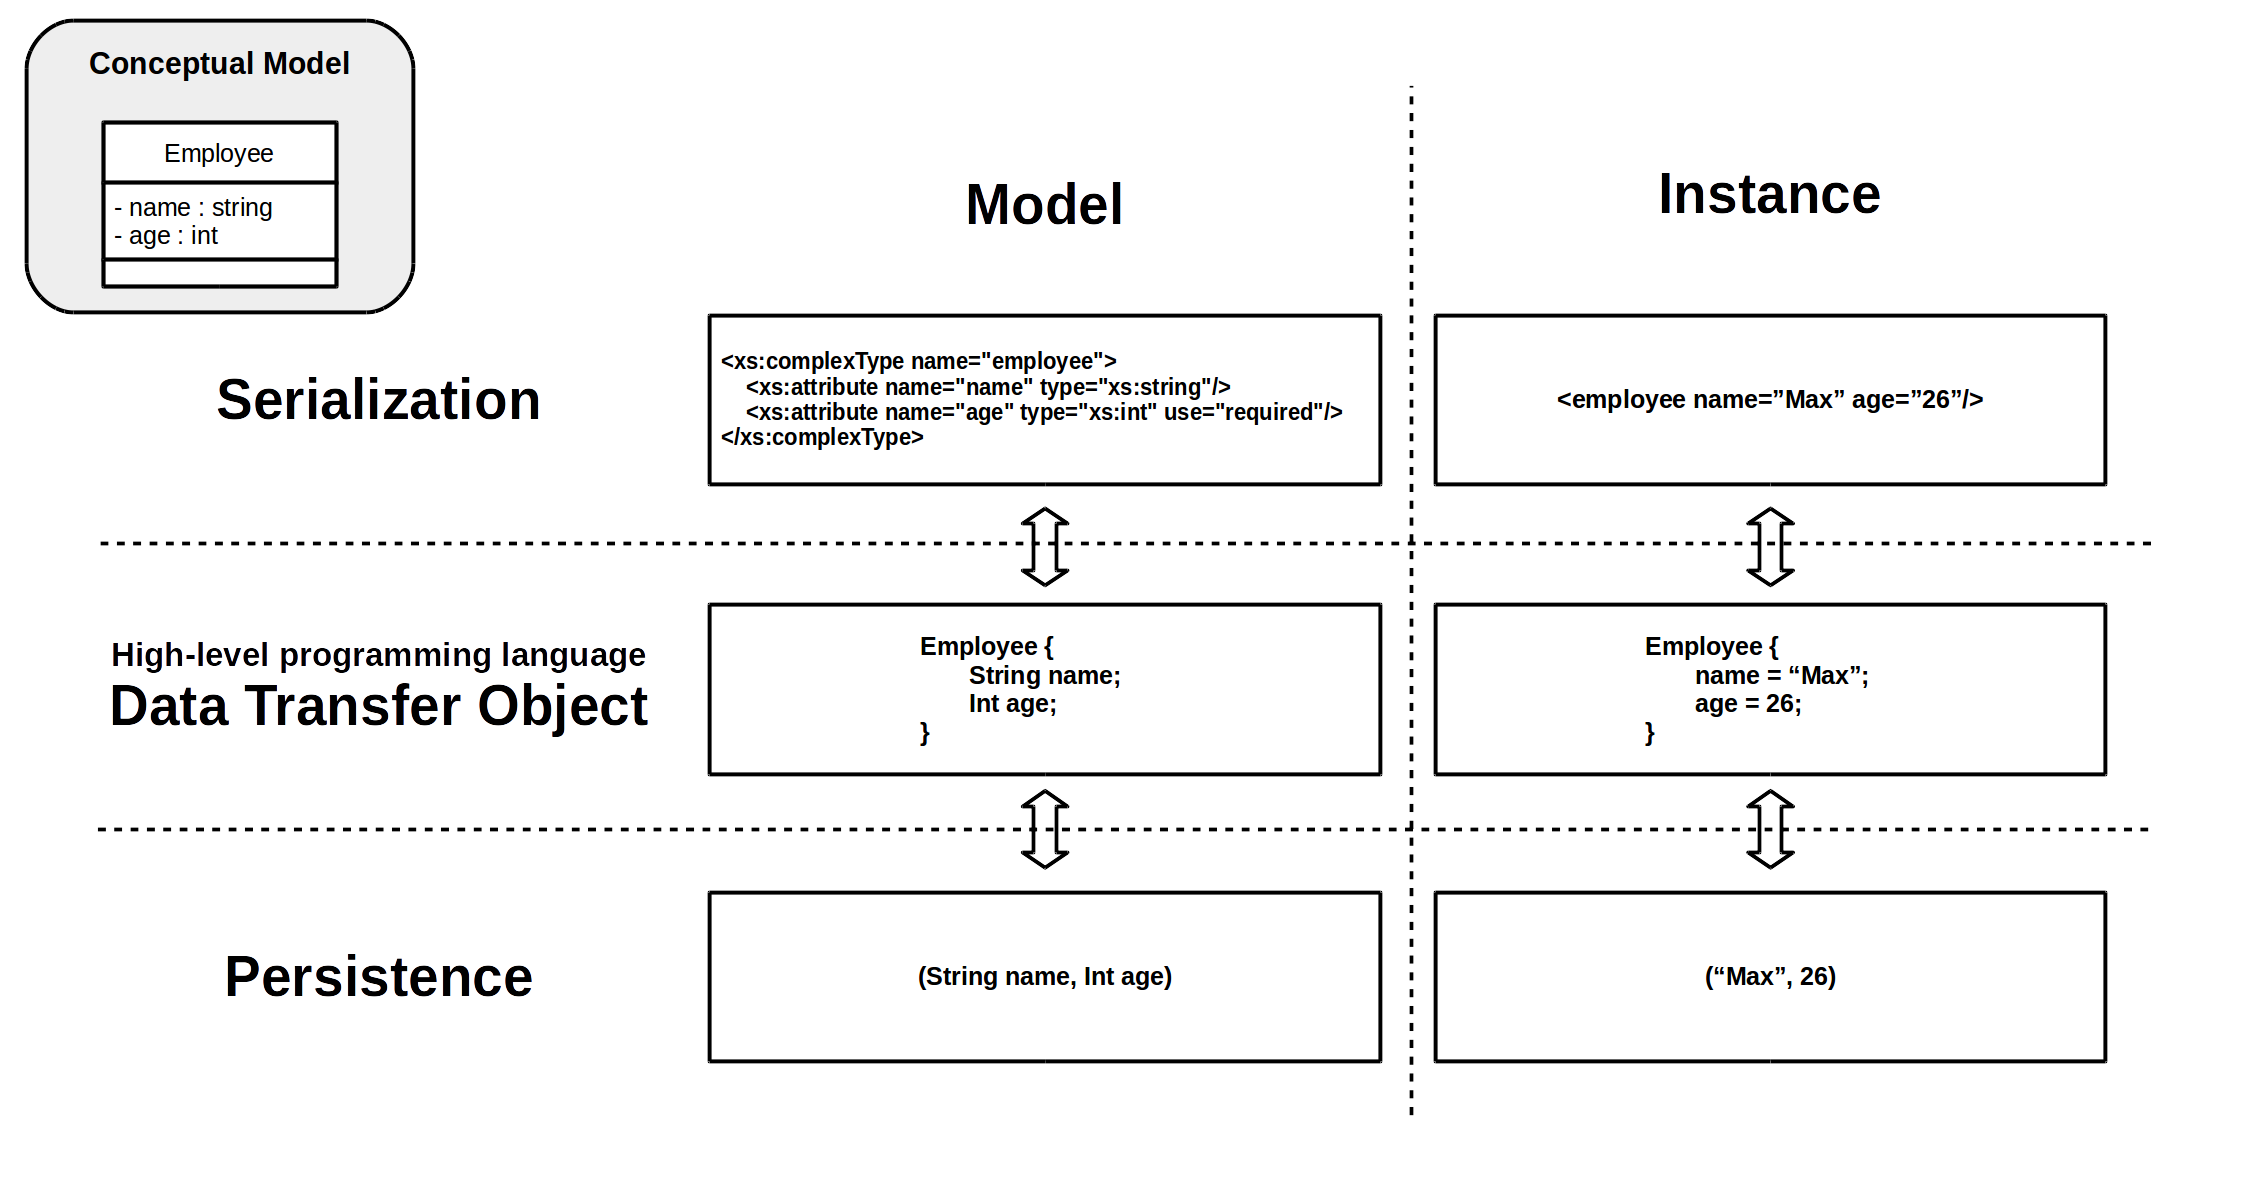
\includegraphics[width=.9\textwidth]{images/ORX.png}
\end{center}
\caption{O/R/X-Mapping Manifestations}
\label{figure:ORXManifestations}
\end{figure}
Figure \ref{figure:ORXManifestations} opposes model- to instance-level syntax of different manifestations for a conceptual model for employees in an \gls{O/R/X-Mapping} scenario.
One employee only has a \textit{name} and an \textit{age} attribute.
Persistence is presented in tuple notation, data transfer objects of an application tier are represented with a fictional high level programming language object notation and serialization is exemplified with \gls{XML} and \gls{XSD} syntax.

Although figure \ref{figure:ORXManifestations} shows a fictionalized example, one can observe structural similarities among the different model and instance representation syntaxes.
Such similarities also occur in real-world software engineering through use of conventions which may be predefined in technologies for \gls{O/R/X-Mapping}.
\begin{figure}[h!]
\begin{center}
\begin{minipage}{.49\textwidth}
\begin{lstlisting}[language=Java,numbers=none]
@XmlRootElement(name="employee")
@XmlAccessorType(XmlAccessType.FIELD)
public class Employee {

	@XmlAttribute
	private int id;
	
	@XmlAttribute
	private String name;
	
	@XmlAttribute
	private int age;
	
	@XmlAttribute
	private double salary;
	
	private Department department;
	
	private Department managedDepartment;
	
}
\end{lstlisting}
\end{minipage}
\hspace*{\fill}
\begin{minipage}{.49\textwidth}
\begin{lstlisting}[language=XML,numbers=none]
<xs:complexType name="employee">
 <xs:attribute name="id" type="xs:int" use="required"/>

 <xs:attribute name="name" type="xs:string"/>

 <xs:attribute name="age" type="xs:int" use="required"/>

 <xs:attribute name="salary" type="xs:double" use="required"/>
 
 <xs:sequence>
 
   <xs:element ref="department" minOccurs="0"/>
 
   <xs:element name="managedDepartment" type="department" minOccurs="0"/>
 
 </xs:sequence>
</xs:complexType>
\end{lstlisting}
\end{minipage}
\begin{minipage}{\textwidth}
\begin{lstlisting}[language=XML,numbers=none]
<employee name="Max" age="26" salary="55000.0"/>
\end{lstlisting}
\end{minipage}
\end{center}
\caption{JAXB XML/XSD Mapping}
\label{figure:JAXBMapping}
\end{figure}
Figure \ref{figure:JAXBMapping} displays an annotated \gls{Java} class and \gls{XML}/\gls{XSD} output generated by \gls{JAXB}.
Except for the root element all names for attributes and elements are taken from the \gls{Java} class.
Moreover, the \gls{XSD} complex type and the \gls{Java} class share a similar nested structure.
Similarities can found within the model level \glspl{Representation} (\gls{Java}-\gls{XSD}) and between model and instance level \glspl{Manifestation} (\gls{Java}-\gls{XML} and \gls{XSD}-\gls{XML}).

The aim of this thesis is to provide automated recovery of such similarities as semantic links.
Recovered links are inserted into \textit{\glspl{Megamodel}} \cite{DBLP:conf/sattose/BaggeZ14} \cite{DBLP:journals/entcs/FavreN05} for \textit{\glspl{LinguisticArchitecture}} \cite{DBLP:conf/models/FavreLV12} \cite{DBLP:conf/ecmdafa/LammelV14} \cite{HeinzLV17}.
\Glspl{Megamodel} are models providing a high level of abstraction with other models as modeling elements, e.g. a \gls{Megamodel} may describe the dependencies between \glspl{Metamodel}, models and instances.
\Glspl{LinguisticArchitecture} intend to describe software systems from a language centric point of view.
They model knowledge about software systems in terms of \glspl{Language}, \glspl{Artifact}, \glspl{Technology}, etc.
Such entities are interrelated with relationships derived from common software engineering and theoretical computer science vocabulary providing special semantics, e.g. \textit{defines}, \textit{isA}, \textit{instanceOf}, \textit{represents}, \textit{implements}, \textit{realizationOf}, \textit{elementOf}, \textit{subsetOf}, etc.

\Glspl{LinguisticArchitecture} are related to \glspl{ERModel} and \glspl{Ontology}.
Recovering semantic links as described above is related to the concept \textit{\gls{Traceability}} and an application of \textit{\gls{TraceabilityRecovery}} \cite{DBLP:books/daglib/p/GotelCHZEGDAMM12}.
In context of \gls{Traceability} semantic links may be called \textit{\gls{TraceLink}}, however, both establish a relation between two entities denoting a certain semantic.

\section{Approach}
\label{section:Approach}


\begin{figure}[h!]
\begin{center}
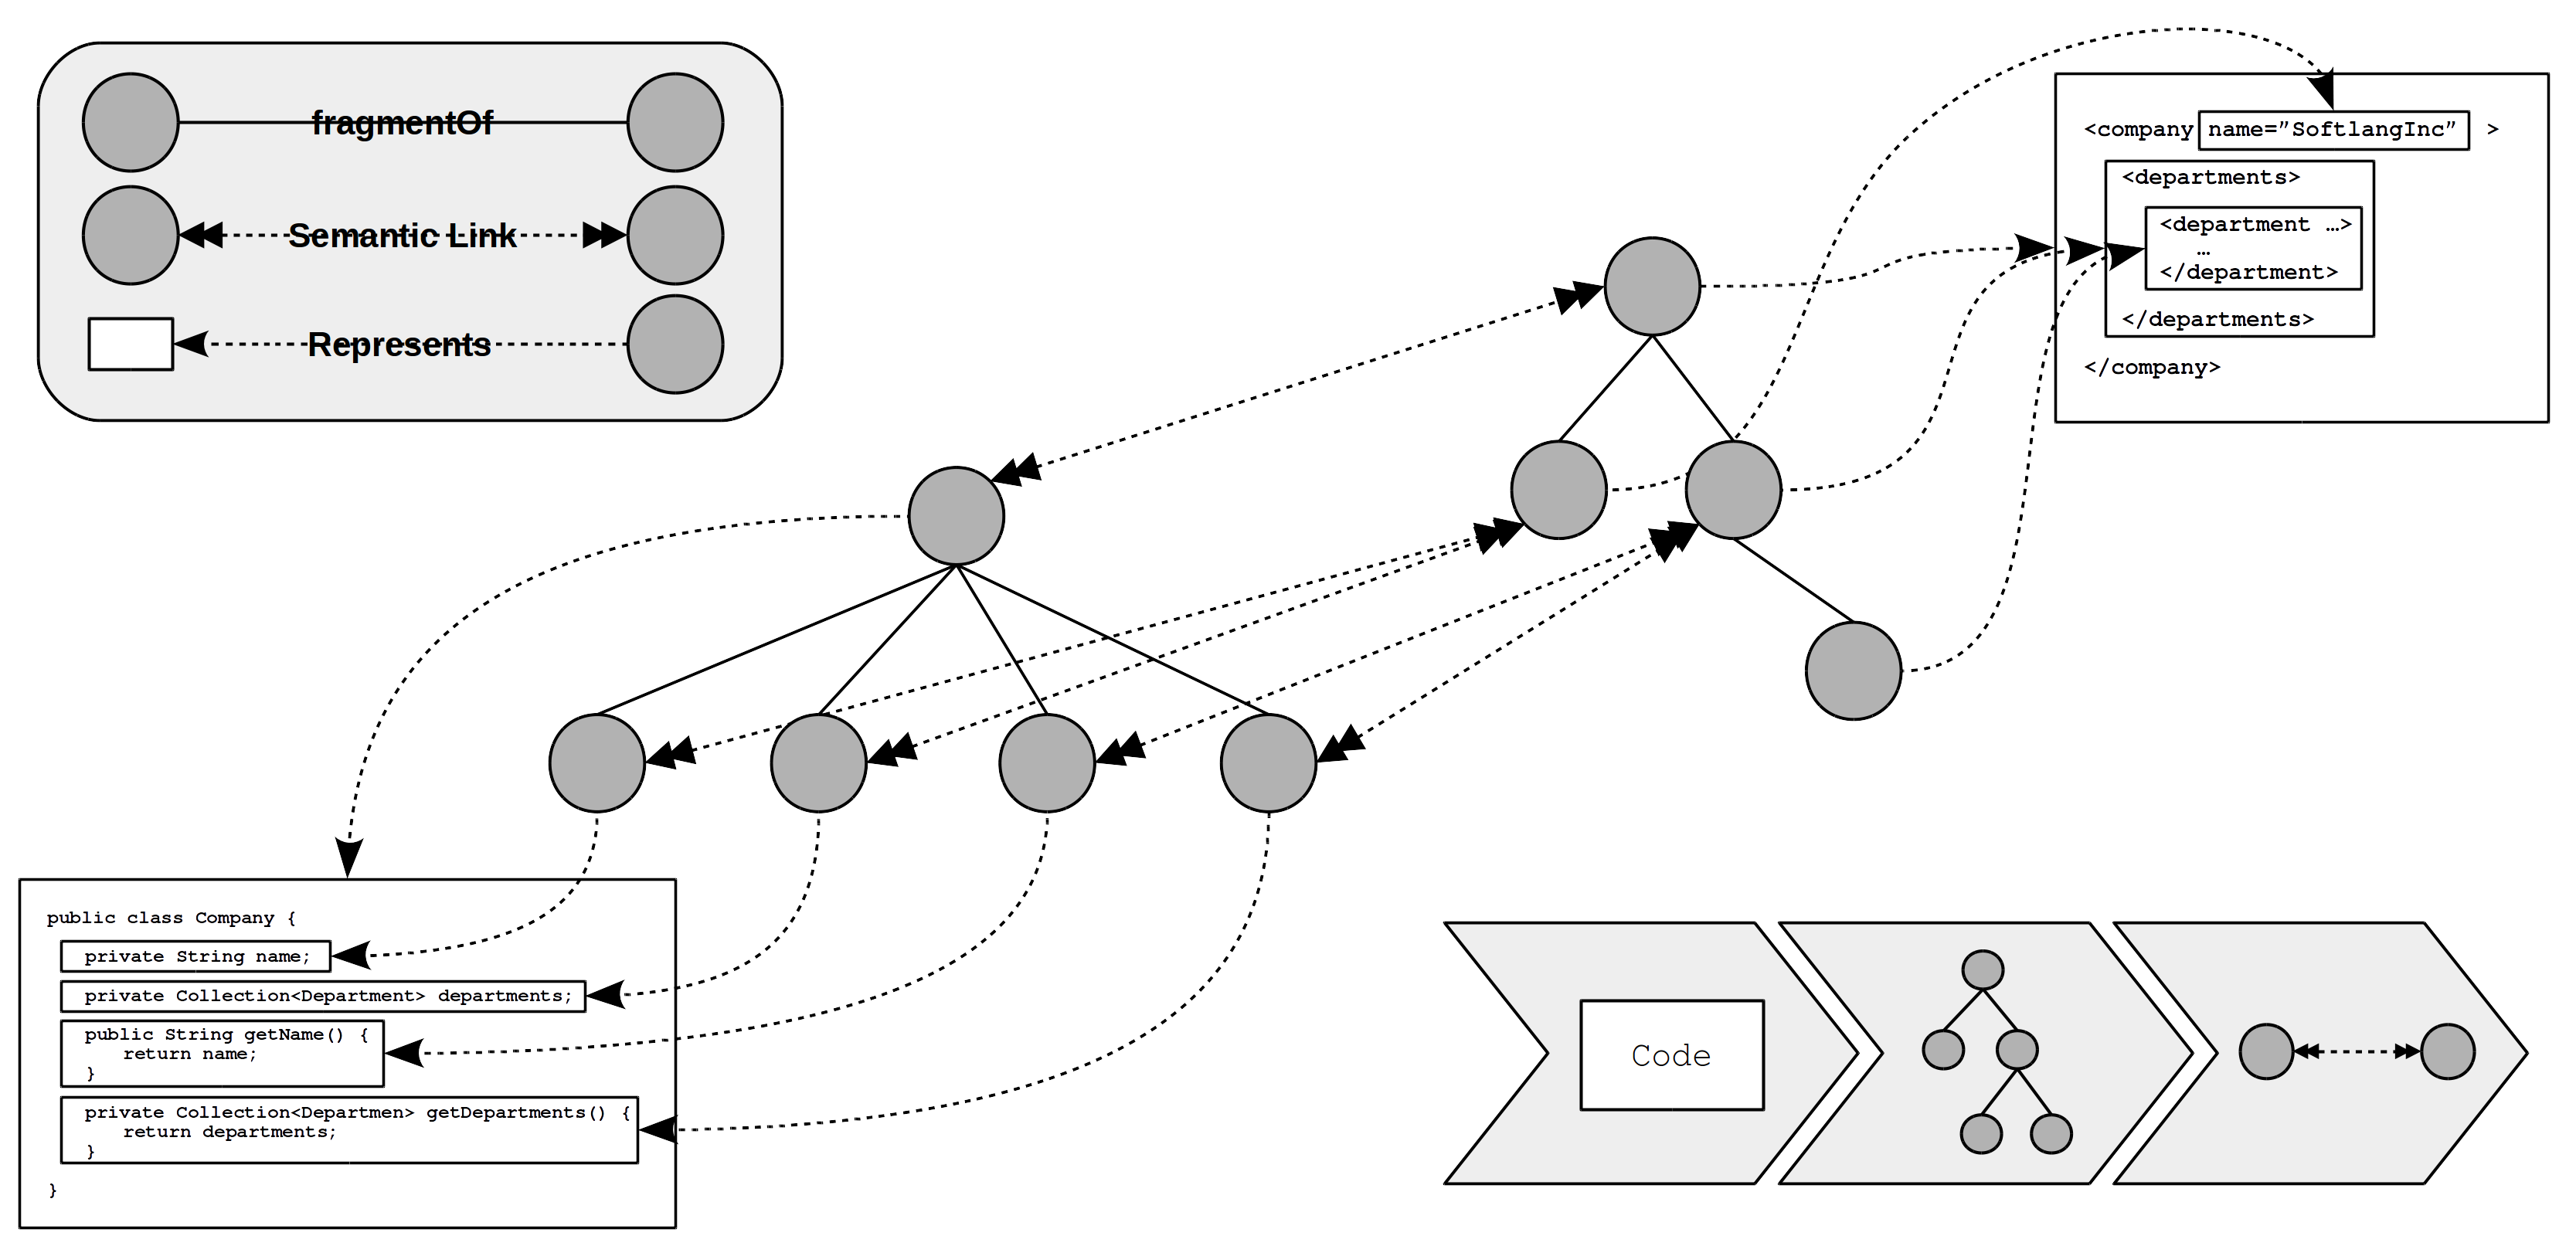
\includegraphics[width=\textwidth]{images/RecoveryExample.png}
\end{center}
\caption{Recovery Approach}
\label{figure:RecoveryApproach}
\end{figure}

\section{Contributions \& Non-Contributions}
\label{section:ContributionsAndNonContributions}
This section lists critical contributions and non-contributions of this thesis:

\begin{contributions}

\item
We contribute a \gls{Java} based \gls{API} for recovering traceability/semantic links among \glspl{Artifact} and their constituent \glspl{Fragment} by means of syntactic analysis (see §\ref{chapter:Design}).

\item
We contribute an implementation of \gls{Correspondence} and \gls{Conformance} link recovery among \gls{JAXB} and \gls{Hibernate} \glspl{Artifact} utilizing the created \gls{API} and axioms for linguistic architectures (see §\ref{chapter:Implementation} and §\ref{section:AxiomsOfLinguisticArchitectures} respectively).

\item
We contribute a small case-study applying the implemented recovery system to a minimal \gls{O/R/X-Mapping} program (see §\ref{chapter:CaseStudy}).

\end{contributions}

\begin{noncontributions}

\item
We do not contribute to the axiomatization of linguistic architectures as described in \cite{DBLP:conf/ecmdafa/LammelV14}, \cite{DBLP:journals/entcs/FavreN05}, \cite{DBLP:conf/sle/Lammel16} and \cite{HeinzLV17}.

\end{noncontributions}

